\textbf{From reading this section:}

\begin{enumerate}
\item
  You will learn that \emph{peeragogy is about peers learning together,
  and teaching each other}
\item
  You will see some different ways in which learning and learning
  activities can be described.
\item
  You will get a sense of why we are writing this handbook!
\end{enumerate}
\subsection{Introduction}

\emph{A healthy process for learning in paragogy consists in a direct
evolution of the four principles of parliamentary democracy: (1) The
right to speak; (2) The right to be heard; (3) The right to listen; (4)
The right to cooperate in the proliferation of options, that is, the
right to ``co-lead'' in the decision-making system.} -- Fabrizio
Terzi\href{http://campus.ftacademy.org/community/mod/groups/topicposts.php?topic=10060\&group\_guid=8500}{}

The idea that we needed a new theory
(\href{http://archive.p2pu.org/general/node/5574/forums/9415\#comment-4054}{which
we called} \emph{paragogy}) arose out of the challenges we faced doing
peer learning. Specifically, we were particularly interested in the
conditions that were required for volunteer contributors to drive an
learning-focused organization's agenda, and improve things for
participating learners and teachers. How could the organization itself
``learn'' and grow, while participants were also learning and becoming
better contributors?

\href{http://archive.p2pu.org/general/node/15138/forums/25213}{As this
idea took form}, we reflected more on how learning and organizations
work. Just like it would be rare for a business to be successful if it
does not take into account the needs and interests of its clients, it is
unlikely for a learning project to be successful if the act of learning
is not somehow relevant for the people doing it.

So,
\href{http://en.wikiversity.org/wiki/File:Paragogy-final.pdf}{paragogy
became a set of proposed principles} for understanding learning (and
working) together. In particular, we focused on the way in which
co-learners shape their learning context together. Paragogy is not a
recipe: its ideas can grow and change to suit the needs of the moment;
\href{http://paragogy.net/ParagogyPaper2}{as it has matured}, it has
become more of an ``approach'' than it is a set of set-in-stone
principles. Again, we look at how people adapt by co-producing a
learning context; so, for example, it would not be easy to build a
"\emph{democratic}" organization without shared understandings like the
points expressed by Fabrizio Terzi, quoted above.

As time goes by, we hope that we can build paragogical tools that will
help people share their skills, and learn while working together. It is
important to learn more about how to invest one's time and energy
efficiently. At present, ``learning'' is often thought of as something
that happens separately from the rest of life (i.e. in school or
university, or perhaps in libraries and cafes). But in fact, learning
and adaptation are dynamic processes which are happening all the time.
The separation of learning from daily life contributes to making
educational goals appear to be very ``distant''. Thus, it would not be
atypical to find someone saying:

\emph{It would be better for me to be a drug dealer than to study
mathematics, since it will take me years and years before the
mathematics study pays off, whereas I can make money selling drugs right
away.}

Paragogy does not say this thinking is ``wrong''. Rather, it looks for
ways to make adaptation of all forms work better: so, if you want to use
paragogy to learn how to become a better drug dealer, we certainly can't
and aren't going to stop you (and, indeed, there are numerous examples
of paragogy coming from organized crime culture all over the world).

The word ``paragogy'' itself is a massive multi-lingual pun. In Greek,
it means "\emph{production}``. In Latin, it also means, roughly, the
kinds of words produced by adding a given prefix or suffix to another
word (so, it is in some sense a pun on its own name!). Its roots
mean''alongside leading", so we either get the sense of a sustained
critical attitude -- if not a subversive leading astray, \emph{a la}
Socrates of the Apology -- or simply of ``teamwork''. Of course, the
basic meaning in English is just ``peer learning'', and, for this
reason, we often pronounce it ``peeragogy'' when we are talking about
its more learning-specific aspects.

It's also riff on the word ``andragogy'', which comes from Malcolm
Knowles. He wrote:

\emph{``. . . andragogy is simply another model of assumptions about
adult learners to be used alongside the pedagogical model of
assumptions, thereby providing two alternative models for testing out
the assumptions as to their `fit' with particular situations.
Furthermore, the models are probably most useful when seen not as
dichotomous but rather as two ends of a spectrum , with a realistic
assumption (about learners) in a given situation falling in between the
two ends''}
(\href{http://openlibrary.org/works/OL10335330W/The\_modern\_practice\_of\_adult\_education}{Knowles,
1980, p. 43}).

We also tried, at least at first, to be similarly non-oppositional with
respect to andragogy:

\emph{``\ldots{} {[}T{]}he most important initial condition in andragogy
seems to be that an adult educator or facilitator is part of the
picture. In a peer-based setting, that may not be the case: we can
easily find examples of learning environments where there is
no''teacher" in the ``classroom''; where, for example, the task of
facilitation is shared among all participants or even encoded in the
learning materials or supportive technologies. Not that one way is more
desirable than another: we simply mean to highlight the fact that the
most basic features of a given learning environment will influence
everything else."}(\href{http://paragogy.net/ParagogyPaper1}{Corneli \&
Danoff, 2011})

Knowles noted many reasons to move to a theory of adult learning that
took the needs of adults into account -- but many of these same reasons
suggest that we need a better theory of peer learning if we are going to
really use it to its full potential. Consider:

\begin{itemize}
\item
  Many people in online learning contexts are NOT taking initiative.
  There is a
  "\href{http://www.useit.com/alertbox/participation\_inequality.html}{90/9/1
  rule}" that says that, online, 1\% of people create content, 9\% edit
  or modify that content, and 90\% view the content without
  contributing. Is this rule fixed? How do we work in a world where the
  rule applies (or shift things, so that it doesn't)?
\item
  If we want to understand human psychological development, we clearly
  need a \emph{social} psychology component.
\item
  While it is generally a good idea for people to take responsibility
  and initiative in their own learning, this does not come cheaply, and
  it is rare to find a ``wise person'' who has all the answers about how
  that should work; instead, we prefer to participate in a broader
  ``Socratic'' discussion around the topic of learning.
\item
  The strange new world of computers is in fact very familiar to some of
  us, who have created some new strategies for learning in these spaces
  -- and we aim to share them here (as well as look at ``low-tech''
  strategies for learning that work just as well).
\end{itemize}
We will next say a few words about some related theories of learning
which bear certain similarities to paragogy/peeragogy (\ldots{} or
\emph{pæragogy} for short) and which can help contextualize it.

\subsection{So\ldots{} how should we spell it??\textbf{}}

As its etymology indicates, ``paragogy'' is a broad and somewhat
abstract term. ``Peeragogy'' attempts to make the term more concrete and
immediately understandable: clearly, \emph{peeragogy is about peers
learning together, and teaching each other}. But when we wish to remind
the reader who ``is in the know'' that things are, in fact, more
complicated, we will style the word ``pæragogy'', as a reminder that we
are really talking about ``peer produced learning'' broadly construed,
and definitely not just about a new model of ``education''!

\subsection{Constructivism and friends}

\href{http://en.wikipedia.org/wiki/Constructivism\_\%28learning\_theory\%29}{\emph{Constructivism}}
is an umbrella term describing several learning theories. The main idea
of constructivism is that learners actively construct (grow, make,
create, build) their own understanding. \emph{Social constructivism}
focuses on interactions among learners. One of its main themes is the
growth of shared collective knowledge in groups and networks. For
example, social constructivism underlies the theory of communities of
practice. While the ground work can be traced to
\href{http://en.wikipedia.org/wiki/Vygotsky}{Vygotsky} (1930s), the
ideas started to gain momentum in the 1970s.
\emph{\href{http://en.wikipedia.org/wiki/Radical\_constructivism\#Constructivist\_trends}{Radical
constructivism}} (also referred to as \emph{Piagetian constructivism})
focuses on how individuals construct knowledge. The term ``radical''
(\href{http://en.wikipedia.org/wiki/Ernst\_von\_Glasersfeld}{von
Glasersfeld}, 1970s) comes from the claim that no knowledge is ever
``perceived through senses'' but all knowledge is built by the learner.

\href{http://en.wikipedia.org/wiki/Enactivism}{\emph{Enactivism}}
emphasizes interaction of learners with the environment. It builds
bridges across divides between different learning theories. In
particular, it resolves seeming contradictions between social and
radical constructivism. It is a more recent branch of constructivism,
with publications beginning in the 1990s.

\href{http://en.wikipedia.org/wiki/Constructionism\_\%28learning\_theory\%29}{\emph{Constructionism}}
focuses on learning via designing and making artefacts. While the theory
is not restricted by the type of artefacts, many of the original
constructionists in the late 1970s and early 1980s worked with computer
software. Therefore, much of constructionism research focuses on
software design as a learning task. In 2000s, the Maker and DIY
movements gained momentum and connected with constructionist ideas.
Constructionism also connects with social media ideas, such as
co-production.

\href{http://en.wikipedia.org/wiki/Connectivism}{\emph{Connectivism}} is
another more recent variant, especially suited to an online context. In
short, connectivism situates learning in the networks of connections
made among individuals, texts, and each other. We have an article about
the practicalities of a MOOC
\href{\%20http://peeragogy.org/connectivism-in-practice-how-to-organize-a-mooc/}{here}.

Pæragogy would tend to prefer a blend of the ``constructionist'' and
``enactivist'' approaches, which would position learners as both
designing and re-constructing their environment, their language, etc..
Neither technology nor environment is trancendental in this approach.
Rather, learning is a form of adaptation, which also includes a
``terraforming'' component -- and the question of what to ``affirm''
through practice becomes very concrete. We continue with this theme
below.

\subsection{Different ways to engage}

Since we are interested in how students (and others) can collaborate in
learning, bringing to their own particular experiences, strengths, and
weaknesses to bear, we ask: ``How can each participant contribute to a
group in their own way? Which kind of activities can we design to
foster''multi-modal" collaborative learning, and how do we assess the
outcomes?"

One approach is to look at the ``multiple different social roles'' which
people take on in educational contexts:

\emph{{[}W{]}e use {[}Ken{]} Wilber's terms to describe a given
\emph{social role}in terms of its\emph{constituent actions}. So for
example, the role of ``being a student'' might be described as follows:
\emph{``}\textbf{\emph{I}}\emph{go to class,}\textbf{\emph{we}}\emph{do
a class project, the objects of concern (``}\textbf{\emph{Its}}\emph{'')
are things I can add to my portfolio or work-record; and
fundamentally}\textbf{\emph{it}}\emph{is all about gaining a
skill.''}This simple background story gives us a notion of role,
persona, or identity: a role that is defined by its constituent actions,
relative a given social context. And here, context is conceived of,
after Nishida, as a ``shared context in motion.''
(}\href{http://oro.open.ac.uk/33221/1/}{Corneli and Mikroyannidis 2012})

By looking at different roles, we begin to get at ``different paths and
modalities of contribution''. In addition, the I/We/Its/It framework can
be used to decouple learning (and learning design) from any fixed cycle
or set of ``stages'' (e.g.
\href{http://www.slideshare.net/GrainneConole/conole-workshop-ascilitefinal}{\emph{Guidance
\& Support}, \emph{Communication \& Collaboration}, \emph{Reflection \&
Demonstration}, \emph{Content \& Activities}} as used by Conole, or the
\emph{Forming}, \emph{Norming}, \emph{Storming}, \emph{Performing}
framework from
\href{http://en.wikipedia.org/wiki/Tuckman\%27s\_stages\_of\_group\_development}{Tuckman}).
This is not to say that those frameworks are not useful -- but they
should not overdetermine our approach to learning design (see comments
by
\href{http://scholar.google.com/scholar?cluster=11211624493583853867\&hl=en\&as\_sdt=0,14}{Lisewski
and Joyce} on another ``staged'' model, namely
\href{http://www.amazon.com/exec/obidos/ISBN=0415335442}{Salmon's
``five-stage e-moderating model''}). This ``decoupled'' or ``lightly
coupled'' frame of analysis is likely to be a useful move if learning is
happening on an ongoing basis among peers, with the learning context
being reshaped and redefined as we go.

Whatever the ``outer'' framework, learning activities can be sorted into
categories like: \emph{Assimilative}, \emph{Information Processing},
\emph{Communicative}, \emph{Productive}, \emph{Experiential},
\emph{Adaptive}
(\href{http://scholar.google.com/scholar?cluster=8288002155802963960\&hl=en\&as\_sdt=0,14}{Oliver
and Conole}, (etc.) -- or in terms of the ``multiples intelligences''
used (see
\href{http://educ732.courseblock.com/wp-content/uploads/2011/05/multiple\_intelligences.jpg}{this
image} from \href{http://educ732.courseblock.com/}{EDUC 732: Educating
for All Children}; per Howard Gardner).

Indeed, much as we would seek to decouple our ``outer'' frame of
analysis from a cycle, the different ``types'' of activities may be very
subject-, activity-, or person-specific. For example, we might ask
participants to code activities in terms of their associated ``mental
state'' (after
\href{http://en.wikipedia.org/wiki/Mihaly\_Csikszentmihalyi}{Csíkszentmihályi}),
rather than their associated ``intelligence'':

\begin{figure}
\href{http://commons.wikimedia.org/wiki/File\%3AChallenge\_vs\_skill.svg}{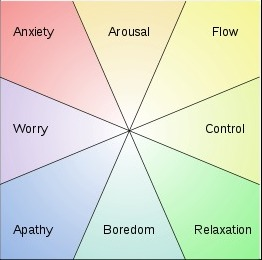
\includegraphics{./pictures/challenge.jpg}}
\caption{
\href{http://commons.wikimedia.org/wiki/File\%3AChallenge\_vs\_skill.svg}{Challenge
vs. Skill}. By w:User:Oliverbeatson (w:File:Challenge vs skill.jpg)
{[}Public domain{]}}
\end{figure}

We could also describe ourselves (or our roles within a learning
process, as above) in terms of various attributes, e.g. using the
proposed framework of Learning Power, with its seven dimensions:
changing and learning -vs- being stuck and static, making meaning -vs-
accumulating data, critical curiosity -vs- passivity, creativity -vs-
being rule-bound, learning relationships -vs- isolation and/or
dependence, strategic awareness -vs- being robotic, resilience -vs-
fragility
(\href{http://scholar.google.com/scholar?cluster=3482923183291547169\&hl=en\&as\_sdt=0,14}{Deakin-Crick,
Broadfoot, and Claxton}).

Similar ideas are summed up in
\href{http://www.amazon.com/Building-Learning-Power-Helping-Learners/dp/1901219437/ref=sr\_1\_1?s=books\&ie=UTF8\&qid=1354332972\&sr=1-1\&keywords=Building+Learning+Power\%3A+Helping+Young+People+Become+Better+Learners}{Claxton's}
four-dimensional framework based on: \emph{resilience},
\emph{resourcefulness}, \emph{reciprocity} and \emph{reflection}.
Whatever framework we use, it is important to remember that, rather than
seeing a person's ``learning power'' in a given situation as an
``essential'' attribute of who they are, one would rather see a person's
overall ``disposition to learning'' as part of an (at least) two-way
relationship
(\href{\%20http://www.umsl.edu/~keelr/3210/resources/PIERREBOURDIEU-KEYTHINK-REV2006.pdf}{Wacquant,
2006} {[}PDF{]}). Thus, peers might use this framework to both better
understand how learning could work in a given situation, and to work
together to devise suitable individual or system-level interventions
that would make it work better.

In sum, we have shown some different ways in which learning and learning
activities can be described. Rather than ``reproducing the system'',
this sort of open-ended descriptive-design process can be used by
learners to identify the topics and ideas of concern to them, as well as
to build their own language, and their own set of social roles, to talk
about and devise methods for addressing issues of concern; cf.
\href{http://scholar.google.com/scholar?cluster=7641713096478524562\&hl=en\&as\_sdt=0,14}{Askins
and Pain}, who write

"\emph{Reading and relating to the research context as a contact zone,
then, necessitates working with and through issues of voice, agency,
power, and desire alongside all participants in the process.}"

What is true of the contact zones in collaborative inquiry research is
if anything even more true for the zones of proximal development we
co-create in peeragogy! The move from merely studying ``peer learning''
to ``doing peeragogy'' is a big step. But of course -- it is one we take
together.

\subsection{Activity}

\emph{tableau vivant}(Interpersonal - Linguistic -- kinesthetical) Ask
participants to create, in groups, a tableau vivant of a given
sequence/scene from a film. Have each person capture a particular
essence/character/situation of the scene. Ask them to freeze their
tableau while the rest of the group observes and identifies the scene,
asking questions, and offering comments and critiques. For a different,
but related, approach try Joe Corneli's
"\href{http://en.wikiversity.org/wiki/User:Arided/ImplementingParagogy}{Implementing
Paragogy}" lesson plan.
